\documentclass[addpoints]{exam}

\printanswers
\CorrectChoiceEmphasis{\color{red}\bfseries}
\usepackage{amssymb, amsmath, amsfonts}
\usepackage{geometry}
\usepackage{graphicx}
\usepackage{tikz}
\usetikzlibrary{calc}
\usepackage{multirow,array} % for payoff matrix formatting
\usepackage[colorlinks,pdfusetitle,urlcolor=blue,citecolor=blue,linkcolor=blue]{hyperref}

\definecolor{crimson}{RGB}{ 170, 4, 36 }
\definecolor{darkblue}{RGB}{ 4, 47, 170 }
\definecolor{brown}{RGB}{ 111, 71, 2 }
\definecolor{periwinkle}{RGB}{ 90, 177, 204 }
\definecolor{ducksgreen}{HTML}{007030}

\geometry{left=1.0in,right=1.0in,top=1.0in,bottom=1.0in}
\pagestyle{headandfoot}
\lhead{EC327 Game Theory}
\chead{Homework 2}
\rhead{Fall 2025}
\runningheadrule

\title{
    \textbf{Econ 327: Game Theory} \\ 
    Homework $\#2$
    }
\author{University of Oregon}
\date{Due: Oct. 10$^{th}$}

% exam-type question formatting
\renewcommand{\thequestion}{\textbf{Q\arabic{question}}}
\bracketedpoints

\begin{document}

\maketitle

\begin{center}
  \gradetable[h][questions]
\end{center}

\vspace{0.5in}

\begin{center}
  \textbf{For homework assignments:}
\end{center}

\begin{itemize}

%  \item DO NOT write your name:
%  this assignment will be graded anonymously. 
%  If you want to, you can include your student ID instead.

  \item Complete \textit{all} questions and parts.

  % I will select one question at random to be graded
  % according to the rubric on Canvas.

  \item You will be graded on not only the content of your work
    but on how clearly you present your ideas.
    Make sure that your handwriting is legible.
    Please use extra pages if you run out of space 
    but make sure that all parts of a question 
    are in the correct order when you submit.

  \item You may choose to work with others,
  but everyone must submit to Canvas individually.

  Please include the names of everyone who you worked with 
  below your own name.
 
\end{itemize}

\vspace{1.0in}

\makebox[.6\textwidth]{Name\enspace\hrulefill}

\vspace{0.5in}

% \begin{center}
%   \fbox{\fbox{\parbox{5.5in}{\centering
%     Answer the questions in the spaces provided on the
%     question sheets. If you run out of room for an answer,
%     continue on the back of the page or another sheet of paper.}}}
% \end{center}

\begin{questions}

\newpage

\question
Imagine a sequential moves version of rock-paper-scissors
where player 2 gets to pick what they will do after player 1 picks.
Please model the game in its extensive form (as a game tree). 
Assume both player 1 and player 2 only care about the result of the game
and have the following preferences over the result of the game:
win $\succ$ tie $\succ$ loss.
\footnote{\href{https://ethanholdahl.com/}{Ethan Holdahl}, University of Oregon}

\begin{parts}
 
  \part[2]
  How many decisions does \textbf{Player 1} have to make in their \textit{complete strategy}?
  In other words, how many \textit{decision nodes} will Player 1 have in the game tree?
  \begin{solution}
    Player 1 only has \textbf{one} decision decision node because they cannot observe Player 2's actions.
  \end{solution}

  \part[2]
  How many decision nodes does \textbf{Player 2} have? Why?

  \begin{solution}
    Player 2 has \textbf{three} decision nodes because they have to make a plan of action for each of the three different strategies they could observe Player 1 choose.
  \end{solution}

  \part[6]
  Draw out the extensive form game.
  Make sure to clearly label all branches, nodes, and choose any payoff values that reflect the preference ranking above.

  \begin{solution}
    \begin{center}
      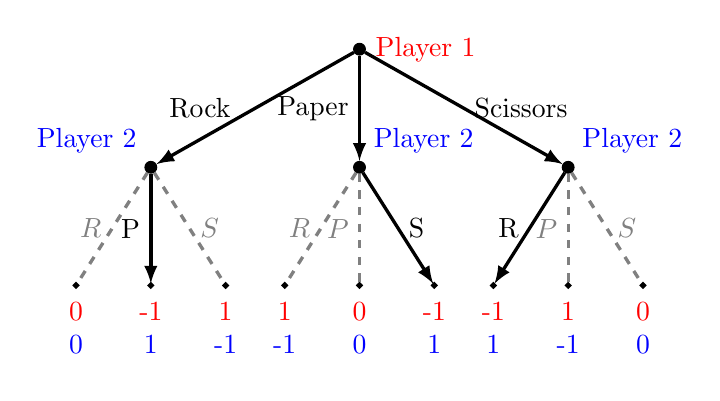
\begin{tikzpicture}[edge from parent/.style={draw, very thick, -latex}]
    \tikzstyle{solid node}=[circle,draw,inner sep=1.5,fill=black]
    \tikzstyle{hollow node}=[circle,draw,inner sep=.25]
    \tikzstyle{level 1}=[level distance=15mm,sibling distance=2.65cm]
    \tikzstyle{level 2}=[level distance=15mm,sibling distance=.95cm]
    \tikzstyle{level 3}=[level distance=15mm,sibling distance=.6cm]
    \tikzstyle{pruned edge from parent}=[draw, very thick, gray, dashed, -]
    
    \node(0)[solid node,label=right:{\color{red} Player 1}]{}
        child{node(1)[solid node,label=above left:{\color{blue} Player 2 }]{}
            child{node[hollow node,label=below:{
                \begin{tabular}{c}
                     {\color{red} 0}  \\
                     {\color{blue} 0} 
                \end{tabular}
            }]{} edge from parent[draw, very thick, gray, dashed, -] node[left]{$R$}}
            child{node[hollow node,label=below:{
                \begin{tabular}{c}
                     {\color{red} -1}  \\
                     {\color{blue} 1} 
                \end{tabular}
            }]{} edge from parent node[left]{P}}
            child{node[hollow node,label=below:{
                \begin{tabular}{c}
                     {\color{red} 1}  \\
                     {\color{blue} -1} 
                \end{tabular}
            }]{} edge from parent[draw, very thick, gray, dashed, -] node[right]{$S$}}
            edge from parent node[left,xshift=-5]{Rock}
        }
        child{node(2)[solid node,label=above right:{\color{blue} Player 2 }]{}
            child{node[hollow node,label=below:{
                \begin{tabular}{c}
                     {\color{red} 1}  \\
                     {\color{blue} -1} 
                \end{tabular}
            }]{} edge from parent[draw, very thick, gray, dashed, -] node[left]{$R$}}
            child{node[hollow node,label=below:{
                \begin{tabular}{c}
                     {\color{red} 0}  \\
                     {\color{blue} 0} 
                \end{tabular}
            }]{} edge from parent[draw, very thick, gray, dashed, -] node[left]{$P$}}
            child{node[hollow node,label=below:{
                \begin{tabular}{c}
                     {\color{red} -1}  \\
                     {\color{blue} 1} 
                \end{tabular}
            }]{} edge from parent node[right]{S}}
            edge from parent node[left]{Paper}
        }
        child{node(3)[solid node,label=above right:{\color{blue} Player 2 }]{}
            child{node[hollow node,label=below:{
                \begin{tabular}{c}
                     {\color{red} -1}  \\
                     {\color{blue} 1} 
                \end{tabular}
            }]{} edge from parent node[left]{R}}
            child{node[hollow node,label=below:{
                \begin{tabular}{c}
                     {\color{red} 1}  \\
                     {\color{blue} -1} 
                \end{tabular}
            }]{} edge from parent[draw, very thick, gray, dashed, -] node[left]{$P$}}
            child{node[hollow node,label=below:{
                \begin{tabular}{c}
                     {\color{red} 0}  \\
                     {\color{blue} 0} 
                \end{tabular}
            }]{} edge from parent[draw, very thick, gray, dashed, -] node[right]{$S$}}
            edge from parent node[right]{Scissors}
        };
\end{tikzpicture}

    \end{center}
  \end{solution}

  \part[6]
  Use \textbf{backwards induction} (rollback) to prune branches which are not sequentially rational.
  Does this game have more than one equilibrium? Why or why not?
  
  \begin{solution}
  In the figure above, dashed lines represent those which have been pruned.

  There are three rollback equilibria because as long as Player 2 chooses whatever action beats Player 1's action,
  Player 1 is indifferent between any of their three strategies.
  Backwards induction cannot be used to prune any of Player 1's strategies, so we must stop here.

  In this case, there are three equilibria:

  \begin{itemize}
      \item $\{$ {\color{red} Rock},     
      {\color{blue} (Paper, Scissors, Rock)} $\}$,
      \item $\{$ {\color{red} Paper},
      {\color{blue} (Paper, Scissors, Rock)} $\}$,
      \item $\{$ {\color{red} Scissors},
      {\color{blue} (Paper, Scissors, Rock)} $\}$
  \end{itemize}
  \end{solution}

\end{parts}

\newpage
\question
  Use the same sequential Rock, Paper, Scissors setup,
  but now imagine player 1's preferences change because they want to be seen as a "tough guy".
  Given that what they want to play remains the same,
  they still have the following preferences over the result of the game:
  win $\succ$ tie $\succ$ loss.
  However, they now would prefer to lose playing rock
  than win playing paper or scissors. 

\begin{parts}
  \part[6]
  Please create a new game tree so the payoffs reflect these new preferences.
  \begin{solution}
    
  I represented Player 1's preferences as:

  payoff to winning with rock = 4,
  tie with rock = 3, 
  lose with rock = 2,
  win with paper or scissors = 1,
  tie with paper or scissors = 0,
  lose with paper or scissors = -1.

  Because payoffs are \textit{ordinal}, 
  you can choose any values as long as the ranking is the same.
  
  \begin{center}
    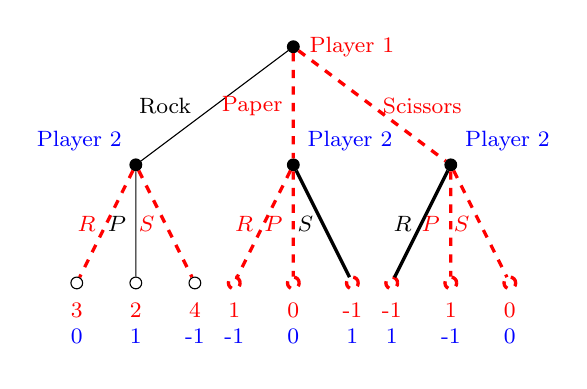
\begin{tikzpicture}[font=\footnotesize]
    \tikzstyle{solid node}=[circle,draw,inner sep=1.5,fill=black]
    \tikzstyle{hollow node}=[circle,draw,inner sep=1.5]
    \tikzstyle{level 1}=[level distance=15mm,sibling distance=2cm]
    \tikzstyle{level 2}=[level distance=15mm,sibling distance=.75cm]
    \tikzstyle{level 3}=[level distance=15mm,sibling distance=.5cm]
    
    \node(0)[solid node,label=right:{\color{red} Player 1}]{}
        child{node(1)[solid node,label=above left:{\color{blue} Player 2 }]{}
            child{node[hollow node,label=below:{
                \begin{tabular}{c}
                     {\color{red} 3}  \\
                     {\color{blue} 0} 
                \end{tabular}
            }]{} edge from parent[red, dashed, very thick] node[left]{$R$}}
            child{node[hollow node,label=below:{
                \begin{tabular}{c}
                     {\color{red} 2}  \\
                     {\color{blue} 1} 
                \end{tabular}
            }]{} edge from parent node[left]{$P$}}
            child{node[hollow node,label=below:{
                \begin{tabular}{c}
                     {\color{red} 4}  \\
                     {\color{blue} -1} 
                \end{tabular}
            }]{} edge from parent[red, dashed, very thick] node[left]{$S$}}
            edge from parent node[left,xshift=-5]{Rock}
        }
        child{node(2)[solid node,label=above right:{\color{blue} Player 2 }]{}
            child{node[hollow node,label=below:{
                \begin{tabular}{c}
                     {\color{red} 1}  \\
                     {\color{blue} -1} 
                \end{tabular}
            }]{} edge from parent[red, dashed, very thick] node[left]{$R$}}
            child{node[hollow node,label=below:{
                \begin{tabular}{c}
                     {\color{red} 0}  \\
                     {\color{blue} 0} 
                \end{tabular}
            }]{} edge from parent[red, dashed, very thick] node[left]{$P$}}
            child{node[hollow node,label=below:{
                \begin{tabular}{c}
                     {\color{red} -1}  \\
                     {\color{blue} 1} 
                \end{tabular}
            }]{} edge from parent[black, solid] node[left]{$S$}}
            edge from parent[red, dashed, very thick] node[left]{Paper}
        }
        child{node(3)[solid node,label=above right:{\color{blue} Player 2 }]{}
            child{node[hollow node,label=below:{
                \begin{tabular}{c}
                     {\color{red} -1}  \\
                     {\color{blue} 1} 
                \end{tabular}
            }]{} edge from parent[black, solid] node[left]{$R$}}
            child{node[hollow node,label=below:{
                \begin{tabular}{c}
                     {\color{red} 1}  \\
                     {\color{blue} -1} 
                \end{tabular}
            }]{} edge from parent[red, dashed, very thick] node[left]{$P$}}
            child{node[hollow node,label=below:{
                \begin{tabular}{c}
                     {\color{red} 0}  \\
                     {\color{blue} 0} 
                \end{tabular}
            }]{} edge from parent[red, dashed, very thick] node[left]{$S$}}
            edge from parent[red, dashed, very thick] node[right]{Scissors}
        };
\end{tikzpicture}

  \end{center}
  \end{solution}

  \part[6]
  Now apply backwards induction to the modified game tree.
  Clearly show on your game tree which branches survive the pruning process.
  \begin{solution}
  Now because Player 1 prefers to lose with rock to any other loss, 
  we can prune the branches where they choose either 
  paper or scissors.
  The only branches which survive pruning are Player 1's Rock and Player 2's Paper after Player 1 chooses Rock.
  \end{solution}

  \part[2]
  What is the rollback equilibrium now?
  
  \begin{solution}
  \{ 
  {\color{red} Rock}, 
  (
  {\color{blue} Paper},
  {\color{blue} Scissors},
  {\color{blue} Rock}
  ) \}

  or in English;
  Player 1 plays Rock,
  Player 2 plays Paper if Player 1 plays Rock,
  Scissors if Player 1 plays Paper,
  and Rock if Player 1 plays Scissors.
  \end{solution}

\end{parts}


%------------------------------------------------------------------

\newpage
\question

At the beginning of the wet season, the herds of gnu which live in the Serengeti migrate South to follow greener grasses.
This is also a prime feeding time for the Nile crocodiles which inhabit the Mara river which the gnu must cross on their way.

To simplify the situation, suppose that there are only two crossings which the gnu can initially approach;
the shallow \textit{rapids}, or the deeper \textit{channel}.
After the gnu arrive at a crossing, suppose the crocodiles can observe where the gnu are gathered and choose which crossing to wait in ambush.

If the gnu cross the river at the same crossing where the crocs are waiting, they are eaten and recieve a payoff of -1.
However, if they cross at the opposite crossing from the crocs, they succesfully cross the river and recieve a payoff of 1.

The crocs want to eat gnu, but they also prefer to wait in the rapids where they can sun themselves rather than the channel.
If the crocs wait in the rapids and they catch the gnu crossing there, the crocs get a payoff of 2.
If the crocs wait in the channel and catch the gnu crossing there, but they only get a payoff of 1.
If the crocs wait in the rapids but they don't catch any gnu, the crocs earn a payoff of 0.
If the crocs wait in the channel but they don't catch any gnu, the crocs get a payoff of -1.

After the gnu have scoped out their choice of crossing, they can choose to either \textit{cross} the river, or \textit{stay} on the banks depending on whether they can see crocs waiting for them.
If the gnu decide to stay on the banks, they get a payoff of 0 (and the crocs don't catch them).

\begin{parts}
  \part[8]
  Draw out the extensive form game. Clearly label all nodes and branches.
  \footnote{Hint: there should be eight possible outcomes.}
  
  \begin{solution}
  \begin{center}
    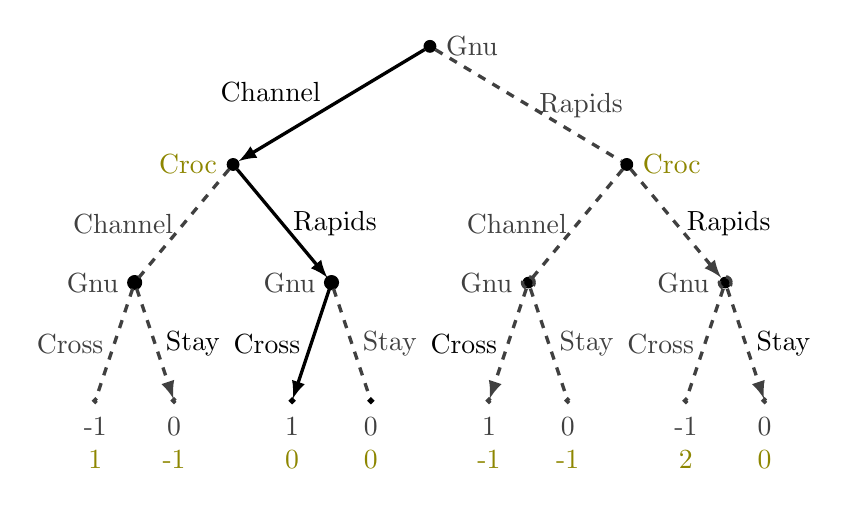
\begin{tikzpicture}[edge from parent/.style={draw, very thick, -latex}]
    \tikzstyle{solid node}=[circle,draw,inner sep=1.5,fill=black]
    \tikzstyle{hollow node}=[circle,draw,inner sep=.25]
    \tikzstyle{level 1}=[level distance=15mm,sibling distance=5cm]
    \tikzstyle{level 2}=[level distance=15mm,sibling distance=2.5cm]
    \tikzstyle{level 3}=[level distance=15mm,sibling distance=1cm]
    \tikzstyle{pruned edge from parent}=[draw, very thick, darkgray, dashed, -]
    
    \node(0)[solid node,label=right:{\color{darkgray} Gnu}]{}
        child{node[solid node,label=left:{\color{olive} Croc }]{}
            child{node[solid node,label=left:{\color{darkgray} Gnu}]{}
                child{node[hollow node,label=below:{
                    \begin{tabular}{c}
                         {\color{darkgray} -1}  \\
                         {\color{olive} 1} 
                    \end{tabular}
                }]{} edge from parent[draw, very thick, darkgray, dashed, -] node[left]{Cross}}
                child{node[hollow node,label=below:{
                    \begin{tabular}{c}
                         {\color{darkgray} 0}  \\
                         {\color{olive} -1} 
                    \end{tabular}
                }]{} edge from parent node[right]{Stay}}
            edge from parent[draw, very thick, darkgray, dashed, -] node[left]{Channel}}
            child{node[solid node,label=left:{\color{darkgray} Gnu}]{}
                child{node[hollow node,label=below:{
                    \begin{tabular}{c}
                         {\color{darkgray} 1}  \\
                         {\color{olive} 0} 
                    \end{tabular}
                }]{} edge from parent node[left]{Cross}}
                child{node[hollow node,label=below:{
                    \begin{tabular}{c}
                         {\color{darkgray} 0}  \\
                         {\color{olive} 0} 
                    \end{tabular}
                }]{} edge from parent[draw, very thick, darkgray, dashed, -] node[right]{Stay}}
            edge from parent node[right]{Rapids}}
            edge from parent node[left,xshift=0,yshift=5]{Channel}
        }
        child{node[solid node,label=right:{\color{olive} Croc }]{}
            child{node[solid node,label=left:{\color{darkgray} Gnu}]{}
                child{node[hollow node,label=below:{
                    \begin{tabular}{c}
                         {\color{darkgray} 1}  \\
                         {\color{olive} -1} 
                    \end{tabular}
                }]{} edge from parent node[left]{Cross}}
                child{node[hollow node,label=below:{
                    \begin{tabular}{c}
                         {\color{darkgray} 0}  \\
                         {\color{olive} -1} 
                    \end{tabular}
                }]{} edge from parent[draw, very thick, darkgray, dashed, -] node[right]{Stay}}
            edge from parent[draw, very thick, darkgray, dashed, -] node[left]{Channel}}
            child{node[solid node,label=left:{\color{darkgray} Gnu}]{}
                child{node[hollow node,label=below:{
                    \begin{tabular}{c}
                         {\color{darkgray} -1}  \\
                         {\color{olive} 2} 
                    \end{tabular}
                }]{} edge from parent[draw, very thick, darkgray, dashed, -] node[left]{Cross}}
                child{node[hollow node,label=below:{
                    \begin{tabular}{c}
                         {\color{darkgray} 0}  \\
                         {\color{olive} 0} 
                    \end{tabular}
                }]{} edge from parent node[right]{Stay}}
            edge from parent node[right]{Rapids}}
            edge from parent[draw, very thick, darkgray, dashed, -] node[right]{Rapids}
        }
        ;
\end{tikzpicture}

  \end{center}
  \end{solution}
  
  \part[8]
  Use backwards induction to solve for the equilibrium.
  \begin{solution}
    Dotted lines in the figure above can be pruned.

    The only equilibrium is where the Gnu Cross only if the Crocs don't choose the same crossing as them.
    The Crocs choose the Rapids no matter what because they know the Gnu will respond by Staying if they follow them and they would rather be in the rapids if they don't get to eat.
    Knowing that the Crocs will stick to the rapids, the Gnu will approach the Channel.
  \end{solution}

\end{parts}
\end{questions}

\end{document}
